%%%%%%%%%%%%%%%%%%%%%%%%%%%%%%%%%%%%%%%%%
% The Legrand Orange Book
% LaTeX Template
% Version 2.4 (26/09/2018)
%
% This template was downloaded from:
% http://www.LaTeXTemplates.com
%
% Original author:
% Mathias Legrand (legrand.mathias@gmail.com) with modifications by:
% Vel (vel@latextemplates.com)
%
% License:
% CC BY-NC-SA 3.0 (http://creativecommons.org/licenses/by-nc-sa/3.0/)
%
% Compiling this template:
% This template uses biber for its bibliography and makeindex for its index.
% When you first open the template, compile it from the command line with the 
% commands below to make sure your LaTeX distribution is configured correctly:
%
% 1) pdflatex main
% 2) makeindex main.idx -s StyleInd.ist
% 3) biber main
% 4) pdflatex main x 2
%
% After this, when you wish to update the bibliography/index use the appropriate
% command above and make sure to compile with pdflatex several times 
% afterwards to propagate your changes to the document.
%
% This template also uses a number of packages which may need to be
% updated to the newest versions for the template to compile. It is strongly
% recommended you update your LaTeX distribution if you have any
% compilation errors.
%
% Important note:
% Chapter heading images should have a 2:1 width:height ratio,
% e.g. 920px width and 460px height.
%
%%%%%%%%%%%%%%%%%%%%%%%%%%%%%%%%%%%%%%%%%

%----------------------------------------------------------------------------------------
%	PACKAGES AND OTHER DOCUMENT CONFIGURATIONS
%----------------------------------------------------------------------------------------

\documentclass[11pt,fleqn]{book} % Default font size and left-justified equations

%%%%%%%%%%%%%%%%%%%%%%%%%%%%%%%%%%%%%%%%%
% The Legrand Orange Book
% Structural Definitions File
% Version 2.1 (26/09/2018)
%
% Original author:
% Mathias Legrand (legrand.mathias@gmail.com) with modifications by:
% Vel (vel@latextemplates.com)
% 
% This file was downloaded from:
% http://www.LaTeXTemplates.com
%
% License:
% CC BY-NC-SA 3.0 (http://creativecommons.org/licenses/by-nc-sa/3.0/)
%
%%%%%%%%%%%%%%%%%%%%%%%%%%%%%%%%%%%%%%%%%

%----------------------------------------------------------------------------------------
%	VARIOUS REQUIRED PACKAGES AND CONFIGURATIONS
%----------------------------------------------------------------------------------------

\usepackage{float}

\usepackage{graphicx} % Required for including pictures
\graphicspath{{Pictures/}} % Specifies the directory where pictures are stored

\usepackage{lipsum} % Inserts dummy text

\usepackage{tikz} % Required for drawing custom shapes

\usepackage[utf8]{inputenc} % Required for including letters with accents
\usepackage[T1]{fontenc} % Use 8-bit encoding that has 256 glyphs

\usepackage{microtype} % Slightly tweak font spacing for aesthetics
\usepackage[ngerman]{babel} % German language/hyphenation
\usepackage[german=quotes]{csquotes}

\usepackage{enumitem} % Customize lists
\setlist{nolistsep} % Reduce spacing between bullet points and numbered lists

\usepackage{booktabs} % Required for nicer horizontal rules in tables

\usepackage{indentfirst}

\usepackage{xcolor} % Required for specifying colors by name
\definecolor{tgmblue}{RGB}{0,162,215} % TGM Blue Arrow
%\definecolor{tgmblue}{RGB}{243,102,25} % Define the orange color used for highlighting throughout the book

%----------------------------------------------------------------------------------------
%	MARGINS
%----------------------------------------------------------------------------------------

\usepackage{geometry} % Required for adjusting page dimensions and margins

\geometry{
	paper=a4paper, % Paper size, change to letterpaper for US letter size
	top=3cm, % Top margin
	bottom=3cm, % Bottom margin
	left=3cm, % Left margin
	right=3cm, % Right margin
	headheight=14pt, % Header height
	footskip=1.4cm, % Space from the bottom margin to the baseline of the footer
	headsep=10pt, % Space from the top margin to the baseline of the header
	%showframe, % Uncomment to show how the type block is set on the page
}

%----------------------------------------------------------------------------------------
%	FONTS
%----------------------------------------------------------------------------------------

\usepackage{avant} % Use the Avantgarde font for headings
%\usepackage{times} % Use the Times font for headings
\usepackage{mathptmx} % Use the Adobe Times Roman as the default text font together with math symbols from the Sym­bol, Chancery and Com­puter Modern fonts

\usepackage{relsize}
\usepackage{textcomp}

%----------------------------------------------------------------------------------------
%	BIBLIOGRAPHY AND INDEX
%----------------------------------------------------------------------------------------

\usepackage[style=numeric,citestyle=numeric,sorting=nyt,sortcites=true,autopunct=true,babel=hyphen,hyperref=true,abbreviate=false,backref=true,backend=biber]{biblatex}
\addbibresource{bibliography.bib} % BibTeX bibliography file
\defbibheading{bibempty}{}

\usepackage{calc} % For simpler calculation - used for spacing the index letter headings correctly
\usepackage{makeidx} % Required to make an index
\makeindex % Tells LaTeX to create the files required for indexing

%----------------------------------------------------------------------------------------
%	MAIN TABLE OF CONTENTS
%----------------------------------------------------------------------------------------

\usepackage{titletoc} % Required for manipulating the table of contents

\contentsmargin{0cm} % Removes the default margin

% Part text styling (this is mostly taken care of in the PART HEADINGS section of this file)
\titlecontents{part}
	[0cm] % Left indentation
	{\addvspace{20pt}\bfseries} % Spacing and font options for parts
	{}
	{}
	{}

% Chapter text styling
\titlecontents{chapter}
	[1.25cm] % Left indentation
	{\addvspace{12pt}\large\sffamily\bfseries} % Spacing and font options for chapters
	{\color{tgmblue!60}\contentslabel[\Large\thecontentslabel]{1.25cm}\color{tgmblue}} % Formatting of numbered sections of this type
	{\color{tgmblue}} % Formatting of numberless sections of this type
	{\color{tgmblue!60}\normalsize\;\titlerule*[.5pc]{.}\;\thecontentspage} % Formatting of the filler to the right of the heading and the page number

% Section text styling
\titlecontents{section}
	[1.25cm] % Left indentation
	{\addvspace{3pt}\sffamily\bfseries} % Spacing and font options for sections
	{\contentslabel[\thecontentslabel]{1.25cm}} % Formatting of numbered sections of this type
	{} % Formatting of numberless sections of this type
	{\hfill\color{black}\thecontentspage} % Formatting of the filler to the right of the heading and the page number

% Subsection text styling
\titlecontents{subsection}
	[1.25cm] % Left indentation
	{\addvspace{1pt}\sffamily\small} % Spacing and font options for subsections
	{\contentslabel[\thecontentslabel]{1.25cm}} % Formatting of numbered sections of this type
	{} % Formatting of numberless sections of this type
	{\ \titlerule*[.5pc]{.}\;\thecontentspage} % Formatting of the filler to the right of the heading and the page number

% Figure text styling
\titlecontents{figure}
	[1.25cm] % Left indentation
	{\addvspace{1pt}\sffamily\small} % Spacing and font options for figures
	{\thecontentslabel\hspace*{1em}} % Formatting of numbered sections of this type
	{} % Formatting of numberless sections of this type
	{\ \titlerule*[.5pc]{.}\;\thecontentspage} % Formatting of the filler to the right of the heading and the page number

% Table text styling
\titlecontents{table}
	[1.25cm] % Left indentation
	{\addvspace{1pt}\sffamily\small} % Spacing and font options for tables
	{\thecontentslabel\hspace*{1em}} % Formatting of numbered sections of this type
	{} % Formatting of numberless sections of this type
	{\ \titlerule*[.5pc]{.}\;\thecontentspage} % Formatting of the filler to the right of the heading and the page number

%----------------------------------------------------------------------------------------
%	MINI TABLE OF CONTENTS IN PART HEADS
%----------------------------------------------------------------------------------------

% Chapter text styling
\titlecontents{lchapter}
	[0em] % Left indentation
	{\addvspace{15pt}\large\sffamily\bfseries} % Spacing and font options for chapters
	{\color{tgmblue}\contentslabel[\Large\thecontentslabel]{1.25cm}\color{tgmblue}} % Chapter number
	{}  
	{\color{tgmblue}\normalsize\sffamily\bfseries\;\titlerule*[.5pc]{.}\;\thecontentspage} % Page number

% Section text styling
\titlecontents{lsection}
	[0em] % Left indentation
	{\sffamily\small} % Spacing and font options for sections
	{\contentslabel[\thecontentslabel]{1.25cm}} % Section number
	{}
	{}

% Subsection text styling (note these aren't shown by default, display them by searchings this file for tocdepth and reading the commented text)
\titlecontents{lsubsection}
	[.5em] % Left indentation
	{\sffamily\footnotesize} % Spacing and font options for subsections
	{\contentslabel[\thecontentslabel]{1.25cm}}
	{}
	{}

%----------------------------------------------------------------------------------------
%	HEADERS AND FOOTERS
%----------------------------------------------------------------------------------------

\usepackage{fancyhdr} % Required for header and footer configuration

\pagestyle{fancy} % Enable the custom headers and footers

\renewcommand{\chaptermark}[1]{\markboth{\sffamily\normalsize\bfseries\chaptername\ \thechapter.\ #1}{}} % Styling for the current chapter in the header
\renewcommand{\sectionmark}[1]{\markright{\sffamily\normalsize\thesection\hspace{5pt}#1}{}} % Styling for the current section in the header

\fancyhf{} % Clear default headers and footers
\fancyhead[LE,RO]{\sffamily\normalsize\thepage} % Styling for the page number in the header
\fancyhead[LO]{\rightmark} % Print the nearest section name on the left side of odd pages
\fancyhead[RE]{\leftmark} % Print the current chapter name on the right side of even pages
%\fancyfoot[C]{\thepage} % Uncomment to include a footer
\fancyfoot[LE]{Lastenheft \emph{Factory Rally}}
\fancyfoot[RO]{tgm | Die Schule der Technik\\ Höhere Lehranstalt für Informationstechnologie}

\renewcommand{\headrulewidth}{0.5pt} % Thickness of the rule under the header
\renewcommand{\footrulewidth}{0.5pt}

\fancypagestyle{plain}{% Style for when a plain pagestyle is specified
	\fancyhead{}\renewcommand{\headrulewidth}{0pt}%
	\fancyfoot{}\renewcommand{\footrulewidth}{0pt}
}

% Removes the header from odd empty pages at the end of chapters
\makeatletter
\renewcommand{\cleardoublepage}{
\clearpage\ifodd\c@page\else
\hbox{}
\vspace*{\fill}
\thispagestyle{empty}
\newpage
\fi}

%----------------------------------------------------------------------------------------
%	THEOREM STYLES
%----------------------------------------------------------------------------------------

\usepackage{amsmath,amsfonts,amssymb,amsthm} % For math equations, theorems, symbols, etc
\usepackage{nccmath}
\usepackage{gensymb}
\usepackage{xfrac}

\newcommand{\intoo}[2]{\mathopen{]}#1\,;#2\mathclose{[}}
\newcommand{\ud}{\mathop{\mathrm{{}d}}\mathopen{}}
\newcommand{\intff}[2]{\mathopen{[}#1\,;#2\mathclose{]}}
\renewcommand{\qedsymbol}{$\blacksquare$}
\newtheorem{notation}{Notation}[chapter]

% Boxed/framed environments
\newtheoremstyle{tgmbluenumbox}% Theorem style name
{0pt}% Space above
{0pt}% Space below
{\normalfont}% Body font
{}% Indent amount
{\small\bf\sffamily\color{tgmblue}}% Theorem head font
{\;}% Punctuation after theorem head
{0.25em}% Space after theorem head
{\small\sffamily\color{tgmblue}\thmname{#1}\nobreakspace\thmnumber{\@ifnotempty{#1}{}\@upn{#2}}% Theorem text (e.g. Theorem 2.1)
\thmnote{\nobreakspace\the\thm@notefont\sffamily\bfseries\color{black}---\nobreakspace#3.}} % Optional theorem note

\newtheoremstyle{blacknumex}% Theorem style name
{5pt}% Space above
{5pt}% Space below
{\normalfont}% Body font
{} % Indent amount
{\small\bf\sffamily}% Theorem head font
{\;}% Punctuation after theorem head
{0.25em}% Space after theorem head
{\small\sffamily{\tiny\ensuremath{\blacksquare}}\nobreakspace\thmname{#1}\nobreakspace\thmnumber{\@ifnotempty{#1}{}\@upn{#2}}% Theorem text (e.g. Theorem 2.1)
\thmnote{\nobreakspace\the\thm@notefont\sffamily\bfseries---\nobreakspace#3.}}% Optional theorem note

\newtheoremstyle{blacknumbox} % Theorem style name
{0pt}% Space above
{0pt}% Space below
{\normalfont}% Body font
{}% Indent amount
{\small\bf\sffamily}% Theorem head font
{\;}% Punctuation after theorem head
{0.25em}% Space after theorem head
{\small\sffamily\thmname{#1}\nobreakspace\thmnumber{\@ifnotempty{#1}{}\@upn{#2}}% Theorem text (e.g. Theorem 2.1)
\thmnote{\nobreakspace\the\thm@notefont\sffamily\bfseries---\nobreakspace#3.}}% Optional theorem note

% Non-boxed/non-framed environments
\newtheoremstyle{tgmbluenum}% Theorem style name
{5pt}% Space above
{5pt}% Space below
{\normalfont}% Body font
{}% Indent amount
{\small\bf\sffamily\color{tgmblue}}% Theorem head font
{\;}% Punctuation after theorem head
{0.25em}% Space after theorem head
{\small\sffamily\color{tgmblue}\thmname{#1}\nobreakspace\thmnumber{\@ifnotempty{#1}{}\@upn{#2}}% Theorem text (e.g. Theorem 2.1)
\thmnote{\nobreakspace\the\thm@notefont\sffamily\bfseries\color{black}---\nobreakspace#3.}} % Optional theorem note
\makeatother

% Defines the theorem text style for each type of theorem to one of the three styles above
\newcounter{dummy} 
\numberwithin{dummy}{section}
\theoremstyle{tgmbluenumbox}
\newtheorem{theoremeT}[dummy]{Theorem}
\newtheorem{problem}{Problem}[chapter]
\newtheorem{exerciseT}{Exercise}[chapter]
\theoremstyle{blacknumex}
\newtheorem{exampleT}{Example}[chapter]
\theoremstyle{blacknumbox}
\newtheorem{vocabulary}{Vocabulary}[chapter]
\newtheorem{definitionT}{Definition}[section]
\newtheorem{corollaryT}[dummy]{Corollary}
\theoremstyle{tgmbluenum}
\newtheorem{proposition}[dummy]{Proposition}

%----------------------------------------------------------------------------------------
%	DEFINITION OF COLORED BOXES
%----------------------------------------------------------------------------------------

\RequirePackage[framemethod=default]{mdframed} % Required for creating the theorem, definition, exercise and corollary boxes

% Theorem box
\newmdenv[skipabove=7pt,
skipbelow=7pt,
backgroundcolor=black!5,
linecolor=tgmblue,
innerleftmargin=5pt,
innerrightmargin=5pt,
innertopmargin=5pt,
leftmargin=0cm,
rightmargin=0cm,
innerbottommargin=5pt]{tBox}

% Exercise box	  
\newmdenv[skipabove=7pt,
skipbelow=7pt,
rightline=false,
leftline=true,
topline=false,
bottomline=false,
backgroundcolor=tgmblue!10,
linecolor=tgmblue,
innerleftmargin=5pt,
innerrightmargin=5pt,
innertopmargin=5pt,
innerbottommargin=5pt,
leftmargin=0cm,
rightmargin=0cm,
linewidth=4pt]{eBox}	

% Definition box
\newmdenv[skipabove=7pt,
skipbelow=7pt,
rightline=false,
leftline=true,
topline=false,
bottomline=false,
linecolor=tgmblue,
innerleftmargin=5pt,
innerrightmargin=5pt,
innertopmargin=0pt,
leftmargin=0cm,
rightmargin=0cm,
linewidth=4pt,
innerbottommargin=0pt]{dBox}	

% Corollary box
\newmdenv[skipabove=7pt,
skipbelow=7pt,
rightline=false,
leftline=true,
topline=false,
bottomline=false,
linecolor=gray,
backgroundcolor=black!5,
innerleftmargin=5pt,
innerrightmargin=5pt,
innertopmargin=5pt,
leftmargin=0cm,
rightmargin=0cm,
linewidth=4pt,
innerbottommargin=5pt]{cBox}

% Creates an environment for each type of theorem and assigns it a theorem text style from the "Theorem Styles" section above and a colored box from above
\newenvironment{theorem}{\begin{tBox}\begin{theoremeT}}{\end{theoremeT}\end{tBox}}
\newenvironment{exercise}{\begin{eBox}\begin{exerciseT}}{\hfill{\color{tgmblue}\tiny\ensuremath{\blacksquare}}\end{exerciseT}\end{eBox}}				  
\newenvironment{definition}{\begin{dBox}\begin{definitionT}}{\end{definitionT}\end{dBox}}	
\newenvironment{example}{\begin{exampleT}}{\hfill{\tiny\ensuremath{\blacksquare}}\end{exampleT}}		
\newenvironment{corollary}{\begin{cBox}\begin{corollaryT}}{\end{corollaryT}\end{cBox}}	

%----------------------------------------------------------------------------------------
%	REMARK ENVIRONMENT
%----------------------------------------------------------------------------------------


\newenvironment{remark}{\par\vspace{10pt}\small % Vertical white space above the remark and smaller font size
\begin{list}{}{
\leftmargin=35pt % Indentation on the left
\rightmargin=25pt}\item\ignorespaces % Indentation on the right
\makebox[-2.5pt]{\begin{tikzpicture}[overlay]
\node[draw=tgmblue!60,line width=1pt,circle,fill=tgmblue!25,font=\sffamily\bfseries,inner sep=2pt,outer sep=0pt] at (-15pt,0pt){\textcolor{tgmblue}{R}};\end{tikzpicture}} % Orange R in a circle
\advance\baselineskip -1pt}{\end{list}\vskip5pt} % Tighter line spacing and white space after remark

%----------------------------------------------------------------------------------------
%	SECTION NUMBERING IN THE MARGIN
%----------------------------------------------------------------------------------------

\usepackage{hyperref}
\hypersetup{hidelinks,backref=true,pagebackref=true,hyperindex=true,colorlinks=false,breaklinks=true,urlcolor=tgmblue,bookmarks=true,bookmarksopen=false}

\makeatletter
\renewcommand{\@seccntformat}[1]{\llap{\textcolor{tgmblue}{\csname the#1\endcsname}\hspace{1em}}}                    
\renewcommand{\section}{\@startsection{section}{1}{\z@}
{-4ex \@plus -1ex \@minus -.4ex}
{1ex \@plus.2ex }
{\normalfont\large\sffamily\bfseries}}
\renewcommand{\subsection}{\@startsection {subsection}{2}{\z@}
{-3ex \@plus -0.1ex \@minus -.4ex}
{0.5ex \@plus.2ex }
{\normalfont\sffamily\bfseries}}
\renewcommand{\subsubsection}{\@startsection {subsubsection}{3}{\z@}
{-2ex \@plus -0.1ex \@minus -.2ex}
{.2ex \@plus.2ex }
{\normalfont\small\sffamily\bfseries}}                        
\renewcommand\paragraph{\@startsection{paragraph}{4}{\z@}
{-2ex \@plus-.2ex \@minus .2ex}
{.1ex}
{\normalfont\small\sffamily\bfseries}}

%----------------------------------------------------------------------------------------
%	PART HEADINGS
%----------------------------------------------------------------------------------------

% Numbered part in the table of contents
\newcommand{\@mypartnumtocformat}[2]{%
	\setlength\fboxsep{0pt}%
	\noindent\colorbox{tgmblue!20}{\strut\parbox[c][.7cm]{\ecart}{\color{tgmblue!70}\Large\sffamily\bfseries\centering#1}}\hskip\esp\colorbox{tgmblue!40}{\strut\parbox[c][.7cm]{\linewidth-\ecart-\esp}{\Large\sffamily\centering#2}}%
}

% Unnumbered part in the table of contents
\newcommand{\@myparttocformat}[1]{%
	\setlength\fboxsep{0pt}%
	\noindent\colorbox{tgmblue!40}{\strut\parbox[c][.7cm]{\linewidth}{\Large\sffamily\centering#1}}%
}

\newlength\esp
\setlength\esp{4pt}
\newlength\ecart
\setlength\ecart{1.2cm-\esp}
\newcommand{\thepartimage}{}%
\newcommand{\partimage}[1]{\renewcommand{\thepartimage}{#1}}%
\def\@part[#1]#2{%
\ifnum \c@secnumdepth >-2\relax%
\refstepcounter{part}%
\addcontentsline{toc}{part}{\texorpdfstring{\protect\@mypartnumtocformat{\thepart}{#1}}{\partname~\thepart\ ---\ #1}}
\else%
\addcontentsline{toc}{part}{\texorpdfstring{\protect\@myparttocformat{#1}}{#1}}%
\fi%
\startcontents%
\markboth{}{}%
{\thispagestyle{empty}%
\begin{tikzpicture}[remember picture,overlay]%
\node at (current page.north west){\begin{tikzpicture}[remember picture,overlay]%	
\fill[tgmblue!20](0cm,0cm) rectangle (\paperwidth,-\paperheight);
\node[anchor=north] at (4cm,-3.25cm){\color{tgmblue!40}\fontsize{220}{100}\sffamily\bfseries\thepart}; 
\node[anchor=south east] at (\paperwidth-1cm,-\paperheight+1cm){\parbox[t][][t]{8.5cm}{
\printcontents{l}{0}{\setcounter{tocdepth}{1}}% The depth to which the Part mini table of contents displays headings; 0 for chapters only, 1 for chapters and sections and 2 for chapters, sections and subsections
}};
\node[anchor=north east] at (\paperwidth-1.5cm,-3.25cm){\parbox[t][][t]{15cm}{\strut\raggedleft\color{white}\fontsize{30}{30}\sffamily\bfseries#2}};
\end{tikzpicture}};
\end{tikzpicture}}%
\@endpart}
\def\@spart#1{%
\startcontents%
\phantomsection
{\thispagestyle{empty}%
\begin{tikzpicture}[remember picture,overlay]%
\node at (current page.north west){\begin{tikzpicture}[remember picture,overlay]%	
\fill[tgmblue!20](0cm,0cm) rectangle (\paperwidth,-\paperheight);
\node[anchor=north east] at (\paperwidth-1.5cm,-3.25cm){\parbox[t][][t]{15cm}{\strut\raggedleft\color{white}\fontsize{30}{30}\sffamily\bfseries#1}};
\end{tikzpicture}};
\end{tikzpicture}}
\addcontentsline{toc}{part}{\texorpdfstring{%
\setlength\fboxsep{0pt}%
\noindent\protect\colorbox{tgmblue!40}{\strut\protect\parbox[c][.7cm]{\linewidth}{\Large\sffamily\protect\centering #1\quad\mbox{}}}}{#1}}%
\@endpart}
\def\@endpart{\vfil\newpage
\if@twoside
\if@openright
\null
\thispagestyle{empty}%
\newpage
\fi
\fi
\if@tempswa
\twocolumn
\fi}

%----------------------------------------------------------------------------------------
%	CHAPTER HEADINGS
%----------------------------------------------------------------------------------------

% A switch to conditionally include a picture, implemented by Christian Hupfer
\newif\ifusechapterimage
\usechapterimagetrue
\newcommand{\thechapterimage}{}%
\newcommand{\chapterimage}[1]{\ifusechapterimage\renewcommand{\thechapterimage}{#1}\fi}%
\newcommand{\autodot}{.}
\def\@makechapterhead#1{%
{\parindent \z@ \raggedright \normalfont
\ifnum \c@secnumdepth >\m@ne
\if@mainmatter
\begin{tikzpicture}[remember picture,overlay]
\node at (current page.north west)
{\begin{tikzpicture}[remember picture,overlay]
\node[anchor=north west,inner sep=0pt] at (0,0) {\ifusechapterimage\includegraphics[width=\paperwidth]{\thechapterimage}\fi};
\draw[anchor=west] (\Gm@lmargin,-9cm) node [line width=2pt,rounded corners=15pt,draw=tgmblue,fill=white,fill opacity=0.5,inner sep=15pt]{\strut\makebox[22cm]{}};
\draw[anchor=west] (\Gm@lmargin+.3cm,-9cm) node {\huge\sffamily\bfseries\color{black}\thechapter\autodot~#1\strut};
\end{tikzpicture}};
\end{tikzpicture}
\else
\begin{tikzpicture}[remember picture,overlay]
\node at (current page.north west)
{\begin{tikzpicture}[remember picture,overlay]
\node[anchor=north west,inner sep=0pt] at (0,0) {\ifusechapterimage\includegraphics[width=\paperwidth]{\thechapterimage}\fi};
\draw[anchor=west] (\Gm@lmargin,-9cm) node [line width=2pt,rounded corners=15pt,draw=tgmblue,fill=white,fill opacity=0.5,inner sep=15pt]{\strut\makebox[22cm]{}};
\draw[anchor=west] (\Gm@lmargin+.3cm,-9cm) node {\huge\sffamily\bfseries\color{black}#1\strut};
\end{tikzpicture}};
\end{tikzpicture}
\fi\fi\par\vspace*{270\p@}}}

%-------------------------------------------

\def\@makeschapterhead#1{%
\begin{tikzpicture}[remember picture,overlay]
\node at (current page.north west)
{\begin{tikzpicture}[remember picture,overlay]
\node[anchor=north west,inner sep=0pt] at (0,0) {\ifusechapterimage\includegraphics[width=\paperwidth]{\thechapterimage}\fi};
\draw[anchor=west] (\Gm@lmargin,-9cm) node [line width=2pt,rounded corners=15pt,draw=tgmblue,fill=white,fill opacity=0.5,inner sep=15pt]{\strut\makebox[22cm]{}};
\draw[anchor=west] (\Gm@lmargin+.3cm,-9cm) node {\huge\sffamily\bfseries\color{black}#1\strut};
\end{tikzpicture}};
\end{tikzpicture}
\par\vspace*{270\p@}}
\makeatother

%----------------------------------------------------------------------------------------
%	LINKS
%----------------------------------------------------------------------------------------

\usepackage{bookmark}
\bookmarksetup{
open,
numbered,
addtohook={%
\ifnum\bookmarkget{level}=0 % chapter
\bookmarksetup{bold}%
\fi
\ifnum\bookmarkget{level}=-1 % part
\bookmarksetup{color=tgmblue,bold}%
\fi
}
}

\newcommand{\bereich}[1]{\noindent \colorbox{tgmblue!20}{\parbox[c]{\dimexpr\textwidth-2\fboxsep}{\textls*{#1}}}}
\newcommand*{\lehrstoffrule}{%
\par\kern\dimexpr.7\itemsep-\parskip-.6\baselineskip\relax%
{\color{tgmblue!50} \hrulefill}%
\par\kern\dimexpr.3\itemsep-.3\parskip-.6\baselineskip\relax%
\vskip 1.5mm%
}
 % Insert the commands.tex file which contains the majority of the structure behind the template

%\hypersetup{pdftitle={Title},pdfauthor={Author}} % Uncomment and fill out to include PDF metadata for the author and title of the book

%----------------------------------------------------------------------------------------

\begin{document}

%----------------------------------------------------------------------------------------
%	TITLE PAGE
%----------------------------------------------------------------------------------------

\begingroup
	\thispagestyle{empty} % Suppress headers and footers on the title page
	\begin{tikzpicture}[remember picture,overlay]
		\node[inner sep=0pt] (background) at (current page.center) {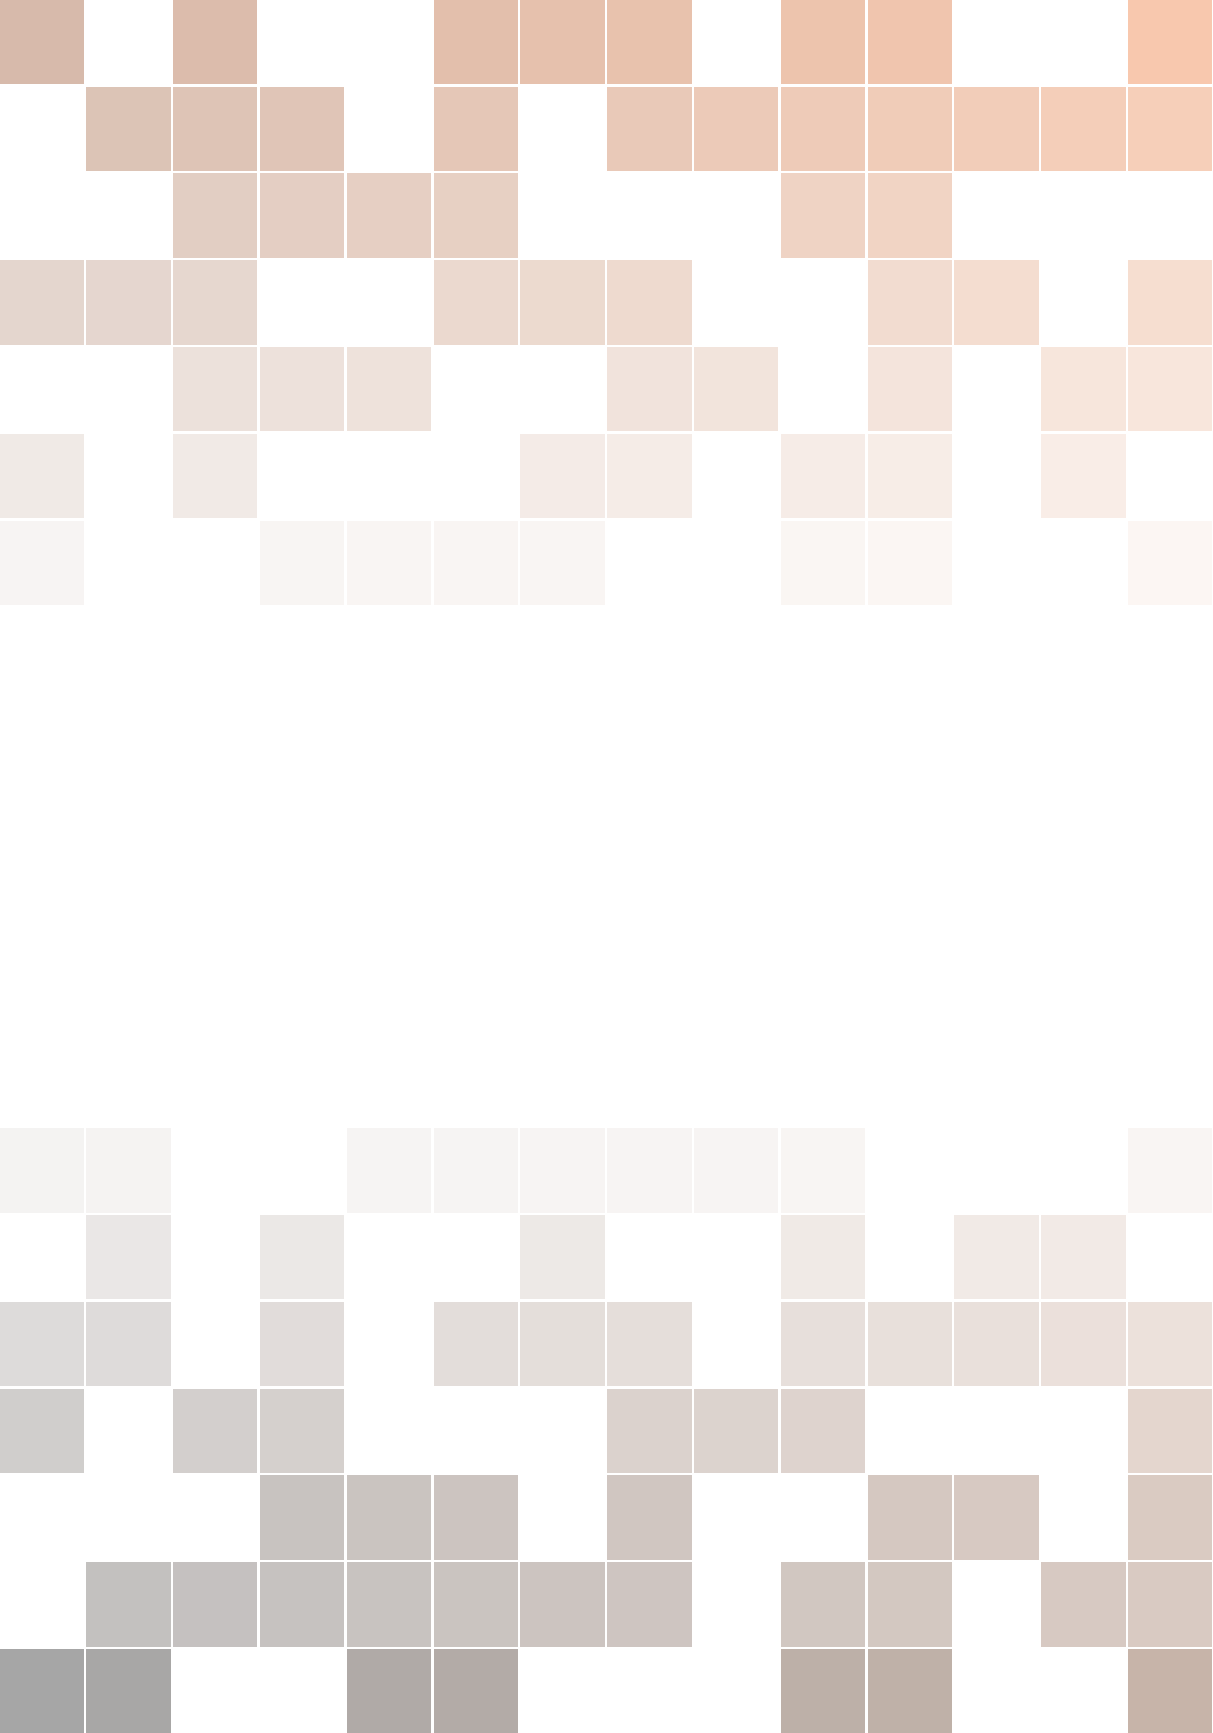
\includegraphics[width=\paperwidth]{background.pdf}};
		\draw (current page.center) node [fill=tgmblue!30!white,fill opacity=0.6,text opacity=1,inner sep=2cm]{\Huge\centering\bfseries\sffamily\parbox[c][][t]{\paperwidth}{
			\centering \textsc{Factory Rally\\[15pt]} % Book title
			{\Large Lastenheft}\\[20pt] % Subtitle
			{\huge Mag. Markus Schabel\\ \LARGE Mag.Dr. Walter Rafeiner-Magor}
		}}; % Author name
		\node[anchor=south,fill=tgmblue!20!white,fill opacity=0.8,inner sep=1.5cm] at (current page.south) {
\begin{tabular}{cccccl}
\textsc{Version} & \textsc{Autor} & \textsc{QS} & \textsc{Datum} & \textsc{Status} & \textsc{Kommentar} \\ \hline
0.1     & SABM & RAFW & \today & Draft & Initialer Entwurf \\
\end{tabular}
		};
	\end{tikzpicture}
	\vfill
\endgroup

%----------------------------------------------------------------------------------------
%	COPYRIGHT PAGE
%----------------------------------------------------------------------------------------

\newpage
~\vfill
\thispagestyle{empty}

\noindent Copyright \copyright\ 2019 Mag. Markus Schabel\\ % Copyright notice

\noindent \textsc{Published by tgm, Abteilung für Informationstechnologie}\\ % Publisher

\noindent \textsc{https://github.com/FactoryRally/lastenheft-global}\\ % URL

\noindent Licensed under the Creative Commons Attribution-NonCommercial 3.0 Unported License (the ``License''). You may not use this file except in compliance with the License. You may obtain a copy of the License at \url{http://creativecommons.org/licenses/by-nc/3.0}. Unless required by applicable law or agreed to in writing, software distributed under the License is distributed on an \textsc{``as is'' basis, without warranties or conditions of any kind}, either express or implied. See the License for the specific language governing permissions and limitations under the License.\\ % License information, replace this with your own license (if any)

\noindent \textit{First printing, Dec. 2019} % Printing/edition date

%----------------------------------------------------------------------------------------
%	TABLE OF CONTENTS
%----------------------------------------------------------------------------------------

%\usechapterimagefalse % If you don't want to include a chapter image, use this to toggle images off - it can be enabled later with \usechapterimagetrue

\chapterimage{chapter_head_1.pdf} % Table of contents heading image

\pagestyle{empty} % Disable headers and footers for the following pages

\tableofcontents % Print the table of contents itself

\cleardoublepage % Forces the first chapter to start on an odd page so it's on the right side of the book

\pagestyle{fancy} % Enable headers and footers again

%----------------------------------------------------------------------------------------
%	PART
%----------------------------------------------------------------------------------------

\part{Lastenheft}

%----------------------------------------------------------------------------------------
%	CHAPTER 1
%----------------------------------------------------------------------------------------

\chapterimage{chapter_head_2.pdf} % Chapter heading image

\chapter{Zielbestimmung}

\emph{RoboRally} ist ein älteres Brettspiel (als 1994), in dem Roboter programmiert werden müssen und ein Spielfeld mit Hindernissen durchlaufen sollen.
Die zugehörige Spielanleitung ist online verfügbar \cite{roborally_rulebook}.
Es gibt bereits digitale Versionen dieses Spiels \cite{roborally_java} sowie eine Implementierung mit \enquote{echten} Robotern  \cite{make_roborally, roboruckus_git, roboruckus_web}.

Ziel dieses Projektes ist es, eine \enquote{moderne} und plattformunabhängige Implementierung dieses Spiels zu realisieren. Diese Implementierung soll aus mehreren Teilen bestehen:

\begin{description}
    \item[Simulierte Umgebung:] die Spielumgebung und die Roboter sollen simuliert werden.
    Die Darstellung kann zweidimensional von oben (z.B. für die Darstellung im Web) oder dreidimensional mit einer Game-Engine (z.B. für mobile Apps oder Desktop Applikationen) realisiert werden.

    \item[Realisierung in Hardware:] die Spielumgebung und die Roboter existieren real, entsprechende Spielbretter und Roboter müssen gefertigt werden.
    Eine entsprechende Überwachung muss stattfinden.
\end{description}

Das Spiel soll in der Simulation mit einem Web-Interface, mit einer mobilen App und mit einer Desktop-Anwendung bedienbar sein.
Spiele sollen von Spielern mit unterschiedlichen Front-Ends gemeinsam gespielt werden können.
In der mobilen App und in der Desktop-Anwendung sollen auch Peer-to-Peer Spiele (d.h. ohne zentralen Server) möglich sein.

Das Spiel in der Hardware-Realisierung soll mit \emph{der gleichen} mobilen App bzw. Desktop-Anwendung bedienbar sein.

Zusätzlich sollen über die Website auch Wettbewerbe geplant und durchgeführt werden können.


\chapter{Produkteinsatz}

TODO


\chapter{Produktfunktionen}

Hier soll ein grober Überblick über die geforderte Funktionalität des Projektes gegeben werden\footnote{diese sind hier bewusst kurz gehalten, da diese als Übung aus den Spielregeln abgeleitet werden sollen}:

\section[Spiel erstellen]{Spiel erstellen\hfill \emph{LF-10}}

Als Spieler möchte ich ein Spiel erstellen (Multiplayer-Spiel, maximale Anzahl von Teilnehmern festlegen, KI-Spieler festlegen, Szenario/Spielbrett auswählen).
    
\section[Spiel beitreten]{Spiel beitreten\hfill \emph{LF-20}}

Als Spieler möchte ich einem Spiel beitreten (ein zufälliges Spiel, ein bestimmtes Spiel mittels z.B. QR-Code o.ä.).
    
\section[Spiel spielen]{Spiel spielen\hfill \emph{LF-30}}

Als Spieler möchte ich ein Spiel bestreiten (in der Simulation: Website, App, Anwendung; in realer Hardware).

\section[Replay ansehen]{Replay ansehen\hfill \emph{LF-40}}

Als Spieler möchte ich ein Replay von einem Spiel ansehen.

\section[An Wettbewerb teilnehmen]{An Wettbewerb teilnehmen\hfill \emph{LF-50}}

Als Spieler möchte ich an einem Wettbewerb teilnehmen und die Ergebnisse sehen.

\section[Wettbewerb erstellen]{Wettbewerb erstellen\hfill \emph{LF-60}}

Als Spielleiter möchte ich einen Wettbewerb erstellen können und diesen auswerten.



\chapter{Produktdaten}

\section[Schnittstellen]{Schnittstellen\hfill \emph{LD-10}}

Das System soll standardisierte Schnittstellen anbieten, damit man \enquote{nach Belieben} neue Front-Ends (Web, App, \dots) bzw. Back-Ends (Hardware, Simulation, KI, \dots) hinzufügen kann.
Als Schnittstelle werden WebServices empfohlen (RESTful, WebSocket, \dots).


\section[Datenformate]{Datenformate\hfill \emph{LD-20}}

Die Daten sollen in standardisierten semistrukturierten Formaten (XML, JSON) ausgetauscht werden.


\section[Datenfluss]{Datenfluss\hfill \emph{LD-30}}


\chapter{Produktcharakteristiken}

\section{Produktionsumgebung}

\subsection{Hardwareumgebung}

Das System und die angeschlossene Hardware sollen auch von Laien einfach installiert und in Betrieb genommen werden.
Die genaue Charakteristik der Hardware wird im Zuge des Projekts evaluiert.


\subsection{Softwareumgebung}

Die Installation des Systems sowie der laufenden Dienste erfolgt automatisch.
Eine Speicherung von Daten erfolgt in entsprechenden Datenbanken.


\section{Entwicklungsumgebung}

Als Entwicklungsumgebung wird die gleiche Hardware wie für die Produktion verwendet, gegebenenfalls um entsprechende Debugging-Interfaces erweitert.
Je nach Auswahl der Hardware muss die passende Softwareumgebung evaluiert werden


\chapter{Nichtfunktionale Anforderungen}

\section[Usability / User eXperience]{Usability / User eXperience\hfill \emph{NF-010}}

Das System bietet ein leicht verständliches Benutzerinterface an und ist auch von Laien einfach bedienbar.

\section[Performance]{Performance\hfill \emph{NF-020}}

Die Responsetime des Systems soll in angemessenen Rahmen sein; es soll eindeutig erkennbar sein, wann das System arbeitet und wann ein Vorgang abgeschlossen ist.

\section[Testing]{Testing\hfill \emph{NF-030}}

Das Testing wird für die einzelnen Module, die Integration der Module sowie für das gesamte System erstellt. Das Testing und deren Ergebnisse werden der Dokumentation beigelegt. Testing wird automatisch durchgeführt (CI/CD).

\section[Code-Qualität]{Code-Qualität\hfill \emph{NF-040}}

Ausgehend von Designideen (Versionierung) wird durch den Einsatz sinnvoller Designmuster ein endgültiges Design erstellt.
Der Sourcecode wird gegen Veränderungen gesichert, für Erweiterungen hingegen offen sein.
Der Sourcecode wird gut und leicht lesbar strukturiert.
Die Namensgebung richtet sich nach den Standards des Anwendungsstack (PHP, JEE, \dots) und verwendet sinnvolle und leicht verständliche Bezeichner.

\section[Dokumentation]{Dokumentation\hfill \emph{NF-050}}

Der Sourcecode wird ausführlich dokumentiert.
Die Standards des Anwendungsstack (JavaDoc, PHPDoc, Sphinx, \dots) werden im Sourcecode verwendet.
Wichtige Stellen im Sourcecode werden ausführlicher dokumentiert.
Ebenso werden komplexere Algorithmen mit einer genauen Dokumentation versehen.
Zusätzlich liegt dem fertigen Sourcecode eine Dokumentation in HTML vor.
Eine übersichtliche Dokumentation der Gesamtarchitektur liegt vor (sowohl der Implementierung als auch der \enquote{zusätzlichen Umgebung} – z.B. CI/CD).

\section[Sicherheit]{Sicherheit\hfill \emph{NF-060}}

Das gesamte System muss vor Angriffen geschützt sein. Dies ist hardwareseitig Roboter), softwareseitig (Schutz für klassischen Angriffen – OWASP) und netzwerkseitig (Schutz vor Netzwerkangriffen, \dots) umzusetzen.
Der Roboter (Hardware) ist sowohl gegen unzulässige Zugriffe (und Programmierungen) abgesichert als auch gegen Verlassen des Spielfeldes (u.ä.).


\chapter{Vertragsgegenstand}

\section{Lieferumfang}

Die Hardware für das System wird fertig (oder zumindest als einfacher Bausatz) ausgeliefert.
Diese ist auch von Laien einfach zu installieren.
Eine ausführliche Dokumentation wird mitgeliefert.

Die Software kann aus den Quellen automatisch erstellt und deployed werden.
Ausführliche Dokumentation auch in Hinsicht auf mögliche Erweiterungen bzw. Folgeprojekte.

\section{Produktbezogene Leistungen}

Das Produkt enthält einen Support.
Der Betreiber der Plattform hat bei Problemen die Möglichkeit mit den Urhebern in Kontakt zu treten und Hilfestellung zu erhalten.
Gegebenenfalls werden Software-Updates zur Verfügung gestellt.


\chapter{Qualitätsanforderungen}

Auf Funktionalität und Zuverlässigkeit wird großer Wert gelegt.

\begin{itemize}
    \item Sicherer Betrieb (hohe Verfügbarkeit, keine „üblichen“ Angriffe möglich)

    \item Einfaches Deployment und Skalierung (paralleler Betrieb in Containern möglich), Verwendung von Testing (auf allen Ebenen) sowie Continuous Integration und Deployment.

    \item Dokumentation insbesondere für Folgeprojekte (Architektur, Patterns, Implementierung, benötigte Umgebung, \dots)
\end{itemize}


%----------------------------------------------------------------------------------------
%	PART
%----------------------------------------------------------------------------------------

\part{Rahmenbedingungen}

%----------------------------------------------------------------------------------------
%	CHAPTER 1
%----------------------------------------------------------------------------------------

\chapterimage{chapter_head_2.pdf} % Chapter heading image

\chapter{Rahmenbedingungen}

Bei der Realisierung des Projekts ist darauf zu achten, dass damit zahlreiche grundlegende und erweiterte Kompetenzen der Fachtheorie-Pflichtgegenstände abgedeckt werden sollen.

Dies betrifft voraussichtlich die im folgenden aufgeführten Gegenstände und Kompetenzen (in der Schulstufe 12 SoSe / 4. Jahrgang Sommersemester).
Angesichts des Projektumfangs ist eine Aufteilung auf mehrere Folgeprojekte durchaus möglich (ggf. auch in anderen Semestern bzw. als Diplomprojekt).


\chapter{Gegenstände}

\section{Softwareentwicklung}

\noindent {\color{red}Grundsätzlich: Verwendung von Frameworks; Dokumentation der Software-Architektur; Verwendung eines öffentlichen Repositories. Offene Schnittstellen vor allem in Hinsicht auf Folgeprojekte.}

\bereich{Anwendungsentwicklung}
\begin{itemize}[label={-}]
    \item Anwendungssysteme unter Verwendung von Nebenläufigkeit entwickeln
        {\color{red}(GUI-Front-End (Desktop/Web/mobile App))};
    \item[] einfache Schnittstellen zur Kommunikation zwischen Anwendungen entwerfen und implementieren
        {\color{red}(Schnittstelle Front-End/Back-End (WebService, WebSocket, REST, \dots))};
    \item[] Programme unter Berücksichtigung von Entwurfsmustern entwickeln
        {\color{red}(GUI Design-Patterns, Observer-Pattern, Command-Pattern, \dots)};
    \item[] Client-Server Anwendungen entwickeln
        {\color{red}(Peer-to-Peer, Client-Server; Front-End/Back-End; \dots)}.
    \item[\tiny\textsc{Lehrstoff}] Definition und Implementierung von Schnittstellen, Threading, Mehrschichtarchitektur, komplexere Entwurfsmuster, Umsetzen von Aufgabenstellungen aus den fachtheoretischen Gegenständen.
\end{itemize}


\section{Informationssysteme}

\bereich{Datenbankanwendungen}

\noindent {\color{red}Korrekte Evaluation / Prototypen für die Machbarkeit von konkreten Datenbank(management)systemen (relational vs. NoSQL) bzw. ORM-Systemen.}

\begin{itemize}[label={-}]
    \item standardisierte Datenbankschnittstellen installieren und konfigurieren, und damit aus gängigen Programmiersprachen mit einem Datenbanksystem kommunizieren
        {\color{red}(Korrekte Evaluation / Prototypen für die Machbarkeit von konkreten Datenbank(management)systemen (relational vs. NoSQL) bzw. ORM-Systemen.)};
    \item[] die Einsatzgebiete von datenbankseitiger Programmierung evaluieren und solche Anwendungen entwickeln
        {\color{red}(Zumindest Einsatz von \enquote{prepared Statements}, insbesondere zur Absicherung der Anwendung)};
    \item[] Anwendungen mit Datenanbindung entwickeln
        {\color{red}(Verwendung passender Technologien, Einsatz von Datenbank-Connectoren bzw. ORM-Systemen)};
    \item[] den Begriff „Transaktion“ erklären, die Voraussetzungen für eine korrekte Abarbeitung nennen sowie die Problematiken bei parallel auftretenden Transaktionen aufzeigen und diese in Fehlerklassen kategorisieren
        {\color{red}(Sinnvolle Absicherung bezüglich gleichzeitiger Datenbankzugriffe)}.
    \item[\tiny\textsc{Lehrstoff}] Aufbau, genormte Datenbank-Schnittstellen, Installation, Konfiguration, Vergleich von Schnittstellen; Einsatzgebiete von Stored Procedures, Trigger, Functions; Zugriff auf Daten aus gängigen Skript- und Programmiersprachen; Isolation Levels, Logs, ACID Kriterien.
\end{itemize}

\bereich{Informationssysteme und Contentmanagement}
\begin{itemize}[label={-}]
    \item die Anforderungen und Klassifizierungen von Informationssystemen angeben;
    \item[] marktgängige Contentmanagementsysteme installieren und konfigurieren
        {\color{red}(Projektwebsite mit Fortschrittsberichten, Projektdokumentation)};
    \item[] Content Management Systeme anwenden, entsprechende Inhalte entwickeln, sowie den entsprechenden Content Livecycle erläutern
        {\color{red}(Webseite für \enquote{langfristiges} Projekt (hinsichtlich von Folgeprojekten, Wartung, \dots); beinhaltet auch Support, Bugtracking, \dots)}.
    \item[\tiny\textsc{Lehrstoff}] Beurteilung marktgängiger Systeme; Installation und Konfiguration und Anwendung von Contentmanagementsystemen. 
\end{itemize}

\bereich{Informationsmanagement}
\begin{itemize}[label={-}]
    \item Informationsschnittstellen implementieren
        {\color{red}(Schnittstelle Roboter-Hardware / Back-End System (?))};
    \item[] die wichtigsten Aspekte in Geschäftsbeziehungen zwischen Unternehmen, Anbietern und Endverbrauchern beschreiben.
    \item[\tiny\textsc{Lehrstoff}] Betriebliche Informationssysteme: Informationsschnittstellen; Geschäftsprozesse: Beziehungen zwischen Anbietern und Endverbrauchern, Beziehungen zwischen Unternehmen.
\end{itemize} 


\section{Medientechnik}

\bereich{Multimedia}
\begin{itemize}[label={-}]
    \item die Grundregeln der Bildgestaltung in der Fotografie technisch korrekt umsetzen sowie Hard- und Software auftretende Probleme analysieren und lösen
        {\color{red}(Projektdokumentation, Benutzermanual, repräsentative Website)};
    \item[] eine projektbezogene Auswahl und Zusammenstellung des zu verwendenden Equipments treffen und mit den entsprechenden Dokumenten die gesamte Logistik (wann/was/wo/wer: Zeitplänen, Drehorte, Raumsetting, Team/Protagonisten) erstellen und anhand von Anforderungen geeignete Software und Techniken auswählen und damit multimediale Projekte umsetzen;
    \item[] Copyright von Bild- und Tonmaterial unterscheiden, derartige Materialien korrekt in Medienprojekten integrieren und mit Bild- und Audioprogrammen bearbeiten;
    \item[] die Schritte von der Idee zur Umsetzung (Präproduktion, Produktion, Postproduktion) erklären und damit eigene Projekte im Team umsetzen
        {\color{red}(Projektdokumentation, Benutzermanual, repräsentative Website)}.
    \item[\tiny\textsc{Lehrstoff}] Bildgestaltung, Filmgestaltung, Audiogestaltung; 3D-Programmierung; Copyright; Präproduktion, Produktion, Postproduktion.\lehrstoffrule
 
    \item eine Fotostrecke zu einem vorgegebenen Thema kreativ und technisch korrekt produzieren
        {\color{red}(Projektdokumentation, Benutzermanual, repräsentative Website)}.
    \item[\tiny\textsc{Lehrstoff}] Visual Storytelling.\lehrstoffrule
 
    \item visuelle Gestaltung in unterschiedlichen Medien umsetzen.
    \item[\tiny\textsc{Lehrstoff}] visuelle Grundelemente, Layout, Gestaltungsmittel.
\end{itemize}

\bereich{Datenbereitstellung, Web- und App-Technologien}
\begin{itemize}[label={-}]
    \item einfache Webapplikationen mit responsiven Designs für unterschiedliche Endgeräte mit client- und serverseitiger Programmierung erstellen
        {\color{red}(Web Front-End)};
    \item[] aus Webapplikationen auf heterogene Datenquellen zuzugreifen.
    \item[\tiny\textsc{Lehrstoff}] Webapplikationen, responsive Design, heterogene Datenquellen.\lehrstoffrule
  
    \item Multimedia-Anwendungen als mobile Applikationen entwickeln;
    \item[] Userinterface-Animationen in einer mobilen Applikation umsetzen
        {\color{red}(mobile App)}.
    \item[\tiny\textsc{Lehrstoff}] Audio- und Video-APIs, GUI-Entwicklung.
\end{itemize}

\bereich{3D-Modellierung, Animation, Interaktion und Simulation}
\begin{itemize}[label={-}]
    \item grundlegende 3D-Postproduktionseffekte erklären und anwenden;
    \item[] gerenderte Bilder in einem genau definierten Format produzieren;
    \item[] eigene Kameras erstellen;
    \item[] eigene 3D-Objekte für andere Anwendungen bereitstellen
        {\color{red}(Simulation in Desktop/mobile App)}.
    \item[] selbst produzierte Grafiken aus einer 3D-Produktion mit Farbmanagement adaptieren und in verschiedene Medien integrieren
        {\color{red}(Projektdokumentation, Benutzermanual, repräsentative Website)}.
    \item[\tiny\textsc{Lehrstoff}] 3D-Postproduktion, Bildformate, Kameras, Datenexport; Farbmanagement, Datenbereitstellung.\lehrstoffrule

    \item mit nichtlinearen Animationstechniken komplexe Szenen erstellen
        {\color{red}(Simulation: Roboter beschleunigt, bremst, \dots)};
    \item[] die Grundlagen von Partikelsystemen erklären
        {\color{red}(Simulation: diverse Hindernisse (Gas), brennender Roboter, \dots)}.
    \item[\tiny\textsc{Lehrstoff}] Nichtlineare Animationen, Partikelsysteme.
\end{itemize}

\bereich{Game Development und Simulation}
\begin{itemize}[label={-}]
    \item Grafikeffekte und Materialien in Game Engines erklären und modifizieren
        {\color{red}(Roboter und Spielfeld; Hindernisse)};
    \item[] Lichter und Beleuchtung in Echtzeitanwendungen erklären und modifizieren
        {\color{red}(Spielfeldbeleuchtung; Lichter; Laser; \dots)};
    \item[] Scripts zur 2D/3D-Simulation erstellen
        {\color{red}(Steuerung der Spielelogik)};
    \item[] Animation von Spielobjekten erstellen
        {\color{red}(Roboter bewegt sich, Elemente am Spielbrett beweglich (z.B. Förderband))};
    \item[] Animation und Gamelogik mittels Programmierung verbinden
        {\color{red}(Implementierung \& Testen)};
    \item[] Co-Routines bzw. Multithreading in Game Scripts einsetzen
        {\color{red}(Multithreading, Roboter mit eigenen Prozessen, \dots)}.
    \item[\tiny\textsc{Lehrstoff}] Physik-Engines, Echtzeit-Grafik, Co-Routines und Threading, Animation.
\end{itemize}

\bereich{Ethische Aspekte, Rechtliche Grundlagen und Gesellschaftliche Auswirkungen der Informationstechnologie -- Basiswissen}
\begin{itemize}[label={-}]
    \item die Interaktion zwischen Informationstechnik, Gesellschaft und Politik beschreiben und erläutern;
    \item[] Kommunikationsfreiheit und Kommunikationsrechte beschreiben und erklären;
    \item[] die Entwicklung und Arbeitsweisen der Datenwirtschaft beschreiben und erläutern;
    \item[] Grundlegende Begriffe der Medienethik nennen und erklären;
    \item[] den Verantwortungsbegriff differenziert beschreiben und erklären;
    \item[] informationsethische und rechtliche Verantwortung im Hinblick auf ihre Erzeugnisse und ihr informationstechnisches Handeln in Beziehung setzen.
    \item[\tiny\textsc{Lehrstoff}] Medienethik.
\end{itemize}


\section{Systemtechnik}

\bereich{Industrielle Informationstechnik}
\begin{itemize}[label={-}]
    \item Sensordaten aufnehmen, aufarbeiten und über gängige industrielle Kommunikationssysteme zur Verfügung stellen
        {\color{red}(Roboter-Hardware: Feststellung des Spielfeldes, Stromverbrauch, Hindernisse, \dots)}.
    \item[\tiny\textsc{Lehrstoff}] Bussysteme, hardwarebasierte Datenaufnahme und -verarbeitung.\lehrstoffrule
 
    \item externe Signale in Roboterprogrammen verarbeiten und Signale an externe Systeme weitergeben
        {\color{red}(Sensorik im Roboter und am Spielfeld; Kommunikation zwischen Roboter und Spielfeld)};
    \item[] Kommunikations-Schnittstellen auswählen, an ein Handhabungssystem koppeln und in Betrieb nehmen
        {\color{red}(Eventuell: Steuerung/Programmierung autonomer Komponenten am Spielfeld)}.
    \item[\tiny\textsc{Lehrstoff}] Erweiterte Teach-In-Programmierung, Kontrollstrukturen, Variablen, Programmstrukturierung, HMI-Anbindung.\lehrstoffrule
 
    \item verschiedene Bewegungsarten des Handhabungssystems anwendungsgerecht kombinieren
        {\color{red}(Eventuell: Steuerung/Programmierung autonomer Komponenten am Spielfeld)};
    \item[] Programme ausführen und mit Hilfe von Teach-In-Techniken und Offlineprogrammierung erstellen und systematisch testen
        {\color{red}(Eventuell: Steuerung/Programmierung autonomer Komponenten am Spielfeld)}.
    \item[\tiny\textsc{Lehrstoff}] Erweiterte Teach-In-Programmierung, Kontrollstrukturen, Variablen, Programmstrukturierung, HMI-Anbindung.
\end{itemize}

\bereich{Systemintegration und Infrastruktur}

\noindent {\color{red}(Ohne passenden Deskriptor im Semester: Realisierung der Back-End Komponenten in Containern.)}
\begin{itemize}[label={-}]
    \item geeignete unternehmensweite Kommunikationsmittel beschreiben, vergleichen, installieren und betreiben
        {\color{red}(Synchrone/Asynchrone Kommunikation zwischen den Spielern (Text/Sprache))};
    \item[] die für Voice over IP benötigten Standards und Protokolle beschreiben sowie geeignete Implementierungen installieren und betreiben
        {\color{red}(Synchrone/Asynchrone Kommunikation zwischen den Spielern (Sprache))}.
    \item[\tiny\textsc{Lehrstoff}] Kommunikationsdienste, Voice over IP.\lehrstoffrule
  
    \item unterschiedliche Zugriffskontrollmechanismen für Systeme vergleichen und Systeme damit geeignet absichern
        {\color{red}(Authentifizierung in Front-End und Back-End; Absicherung der Roboter-Hardware (keine \enquote{anonyme} Programmierung))};
    \item[] verschiedene Firewall-Typen beschreiben und geeignete Systeme in einer Topologie an geeigneter Stelle einsetzen, konfigurieren und betreiben
        {\color{red}(Back-End geeignet absichern)}.
    \item[\tiny\textsc{Lehrstoff}] Access Control, Firewall.
\end{itemize}

\bereich{Dezentrale Systeme}
\begin{itemize}[label={-}]
    \item in dokumentenbasierten dezentralen Systemen eingesetzte offene Dokumentenformate und Auszeichnungssprachen zur Realisierung solcher Systeme einsetzen
        {\color{red}(Datenübertragung zwischen Front-End(s) und Back-End)}.
    \item[\tiny\textsc{Lehrstoff}] Enterprise-Frameworks, Dokumentenorientierte Middleware Systeme, Einsatz von NoSQL/REST/JSON.\lehrstoffrule
  
    \item ein dokumentorientiertes Middleware Systemen konzipieren und implementieren
        {\color{red}(vermutlich eher Nachrichtenorientiert? Eventuell für Leaderboard, Meisterschaften, \dots)}.
    \item[\tiny\textsc{Lehrstoff}] Enterprise-Frameworks, Dokumentenorientierte Middleware Systeme.\lehrstoffrule

    \item ein dezentrales System mit Hilfe von webbasierten Frameworks umsetzen
        {\color{red}(Peer-to-Peer bzw. Client-Server Anwendung)}.
    \item[\tiny\textsc{Lehrstoff}] Enterprise-Frameworks, Einsatz von NoSQL/REST/JSON, Konfiguration und Datenübertragung mittels gängigen Dokumentenformaten.\lehrstoffrule
  
    \item Programmiertechniken in verteilten Systemen zur Realisierung von entfernten Prozeduren, Methoden und Objekten anwenden
        {\color{red}(Peer-to-Peer bzw. Client-Server Anwendung)}.
    \item[\tiny\textsc{Lehrstoff}] Enterprise-Frameworks, Einsatz von entfernten Prozeduren und verteilten Objekten, Konfiguration und Datenübertragung mittels gängigen Dokumentenformaten.
\end{itemize}

\bereich{Ethische Aspekte, Rechtliche Grundlagen und Gesellschaftliche Auswirkungen der Informationstechnologie -- Basiswissen}
\begin{itemize}[label={-}]
    \item die Interaktion zwischen Informationstechnik, Gesellschaft und Politik beschreiben und erläutern;
    \item[] Kommunikationsfreiheit und Kommunikationsrechte beschreiben und erklären;
    \item[] die Entwicklung und Arbeitsweisen der Datenwirtschaft beschreiben und erläutern;
    \item[] Grundlegende Begriffe der Datenethik nennen und erklären;
    \item[] den Verantwortungsbegriff differenziert beschreiben und erklären;
    \item[] informationsethische und rechtliche Verantwortung im Hinblick auf ihre Erzeugnisse und ihr informationstechnisches Handeln in Beziehung setzen.
    \item[\tiny\textsc{Lehrstoff}] Datenethik.
\end{itemize}


\section{Informationstechnische Projekte}

\bereich{Durchführung informationstechnischer Projekte}
\begin{itemize}[label={-}]
    \item Teile des Lastenheft und einer Evaluation selbständig für ein Projekt erstellen
        {\color{red}(Lastenheft anhand der Spielregeln vervollständigen)};
    \item[] Teile einer Evaluation selbständig für ein Projekt erstellen
        {\color{red}(Prototypen für verschiedene Technologien: DB (relational vs. NoSQL, welches ORM) -- Sprache FE/BE (Java/Kotlin; Objective-C/Swift; Java/Python/Node.js/\dots) -- Welcher Controller für Hardware? Welche Sensoren? -- Frameworks für Frontends (Web/App/Desktop)? -- Engine für Simulation (3D, Physik, \dots))};
    \item[] Teile der Useranforderungen entsprechend der gewählten agilen Projektmanagementmethode erstellen
        {\color{red}(Siehe Lastenheft; anhand der konkreten Spielregeln Erstellung von Arbeitspaketen unter Berücksichtigung der daran hängenden Kompetenzen der Fachtheoretischen Gegenstände)};
    \item[] eine korrekte und zeitnahe Aufzeichnung der eigenen Arbeitspakete bzw. Useranforderungen erstellen
        {\color{red}(Siehe Lastenheft; anhand der konkreten Spielregeln Erstellung von Arbeitspaketen unter Berücksichtigung der daran hängenden Kompetenzen der Fachtheoretischen Gegenstände)};
    \item[] mittels Projektpräsentation die eigenen Aufgaben sowie Inhalte und Status des Projektes überzeugend darstellen; einen aktuellen Statusbericht des Projektes erstellen
        {\color{red}(Präsentation auch beim Tag der offenen Tür; Präsentation an \enquote{Folgeklassen} (auch für Folgeprojekte))}.
    \item[\tiny\textsc{Lehrstoff}] Planung und Realisierung informationstechnischer Projekte unter Wahrnehmung typischer Rollenbilder und unter Berücksichtigung von Themenbereichen der technischen Pflichtgegenstände mittels agilen Projektmanagementmethoden.
\end{itemize}

\bereich{Projektmanagement}
\begin{itemize}[label={-}]
    \item Grundlagen der Aufwandschätzung erklären und auf Basis eines Projektes eine passende Variante auswählen
        {\color{red}(Aufwandsschätzung für einzelne Arbeitspakete unter Berücksichtigung der zu erreichenden Kompetenzen)};
    \item[] wesentliche Projektrisiken und Chancen erkennen und geeignete Maßnahmen dafür vorsehen
        {\color{red}(Risikomanagement)};
    \item[] Kreativitätsmethoden von Kreativitätstechniken unterscheiden und den kreativen Prozess beschreiben;
    \item[] Projektkrise und die Begriffe erklären, sowie unterschiedliche Ursachen und Indikatoren für Krisen beschreiben.
    \item[\tiny\textsc{Lehrstoff}] Projektplanung, Projektrisiko, Projektdokumentation, Multiprojektmanagement, Kreativität einsetzen, Krisen analysieren.
\end{itemize}


\section{IT-Sicherheit -- MEDT}

\bereich{Secure Web- \& App-Development}
\begin{itemize}[label={-}]
    \item Web-Anwendungen und mobile Applikationen absichern
        {\color{red}(Absicherung Front-End (und Back End?))};
    \item[] rechtliche Grundlagen erklären und bei der Entwicklung berücksichtigen
        {\color{red}(Datenschutz, Zertifikate, Verschlüsselung)}.
    \item[\tiny\textsc{Lehrstoff}] OWASP Top 10, Web-Application-Firewalls, Datenschutz, Urheberrecht, Zertifikate, Verschlüsselung.
\end{itemize}


\section{IT-Sicherheit -- SYT}

\bereich{IT-Security}
\begin{itemize}[label={-}]
    \item Prinzipien von Penetrationstests erläutern und im rechtlichen Rahmen entsprechende Angriffe durchführen
        {\color{red}(Testen von Back-End und Peer-to-Peer Front-Ends)}.
    \item[\tiny\textsc{Lehrstoff}] Permission-to-Attack, Responsible Disclosure, Data-Privacy.\lehrstoffrule
 
    \item Systeme und deren Schnittstellen gegen Angriffe schützen und härten
        {\color{red}(Absicherung von Front End und Back End)}.
    \item[\tiny\textsc{Lehrstoff}] Buffer-Overflows, Mandatory-Access-Control, Trusted-Platform; IDS, IPS; Datenintegrität; Fuzzing.
\end{itemize}


\section{Artificial Intelligence -- MEDT}

\bereich{Grundlagen der Künstlichen Intelligenz}
\begin{itemize}[label={-}]
    \item Algorithmen der KI erkennen und erstellen
        {\color{red}(Möglichkeiten für KI-gesteuerte Roboter evaluieren)};
    \item[] Systeme zum autonomen Agieren mit Benutzern entwickeln
        {\color{red}(\enquote{Support-Bot} auf Website?)};
    \item[] einfache prozedurale und KI basierte Generierung von Medieninhalten erstellen
        {\color{red}(Automatische Erstellung von: Spielfeldern; Robotern)}.
    \item[\tiny\textsc{Lehrstoff}] KI in Game Engines, Finite State Machines, Suchalgorithmen und deren Anwendungen, Grundlagen Machine Learning und Klassifikation, prozedurale Content-Erstellung.
\end{itemize}


\section{Artificial Intelligence -- SYT}

\bereich{Data Science}
\begin{itemize}[label={-}]
    \item die Qualität von Daten und Algorithmen anhand von Output-Daten überprüfen
        {\color{red}(Festsetzung geeigneter Kriterien für die nachträgliche Auswertung des Projektes (insbesondere Auswertung von Spielern und Spielen); ggf. Einführung eines entsprechenden Scoring-Systems)}.
    \item[\tiny\textsc{Lehrstoff}] Ablauf von Datenanalyse oder maschinellen Lernprozessen durch Exploration; Daten in Trainings- und Testdatensätze aufteilen; Kenntnis von In-sample Schätzungen und Prädiktionen und Out-of-sample Schätzungen und Prädiktionen; Qualitätsprüfung von Algorithmen (z.B. mittels K-facher Kreuz-Validierung); Probleme der Modellanpassung (z.B. Overfitting, Underfitting).\lehrstoffrule
 
    \item gelernte Methoden im Rahmen aktueller Anwendungsgebiete umsetzen
        {\color{red}(Auswertung ähnlicher Daten (Auswertung von Wettbewerben, Spielern, \dots) z.B. auch bei Schach oder Go (weil vielfältige Daten verfügbar))}.
    \item[\tiny\textsc{Lehrstoff}] Umsetzung von Lernprozessen mithilfe von Algorithmen mit dem Ziel der Musterkennung: Kenntnis von Konzepten von Distanzmaßen (z.B. lineare Diskriminanzanalyse, Cluster Analyse (k-nearest neighbors, model based Clustering), Support Vector Machines); Fallstudie: Anwendung von Methoden der Exploration, Modellierung und Qualitätsprüfung anhand eines realen Datensatzes oder einer realen Fallstudie.
\end{itemize}



%%----------------------------------------------------------------------------------------
%	PART
%----------------------------------------------------------------------------------------

\part{Part One}

%----------------------------------------------------------------------------------------
%	CHAPTER 1
%----------------------------------------------------------------------------------------

\chapterimage{chapter_head_2.pdf} % Chapter heading image

\chapter{Text Chapter}

\section{Paragraphs of Text}\index{Paragraphs of Text}

\lipsum[1-7] % Dummy text

%------------------------------------------------

\section{Citation}\index{Citation}

This statement requires citation \cite{article_key}; this one is more specific \cite[162]{book_key}.

%------------------------------------------------

\section{Lists}\index{Lists}

Lists are useful to present information in a concise and/or ordered way\footnote{Footnote example...}.

\subsection{Numbered List}\index{Lists!Numbered List}

\begin{enumerate}
\item The first item
\item The second item
\item The third item
\end{enumerate}

\subsection{Bullet Points}\index{Lists!Bullet Points}

\begin{itemize}
\item The first item
\item The second item
\item The third item
\end{itemize}

\subsection{Descriptions and Definitions}\index{Lists!Descriptions and Definitions}

\begin{description}
\item[Name] Description
\item[Word] Definition
\item[Comment] Elaboration
\end{description}

%----------------------------------------------------------------------------------------
%	CHAPTER 2
%----------------------------------------------------------------------------------------

\chapter{In-text Elements}

\section{Theorems}\index{Theorems}

This is an example of theorems.

\subsection{Several equations}\index{Theorems!Several Equations}
This is a theorem consisting of several equations.

\begin{theorem}[Name of the theorem]
In $E=\mathbb{R}^n$ all norms are equivalent. It has the properties:
\begin{align}
& \big| ||\mathbf{x}|| - ||\mathbf{y}|| \big|\leq || \mathbf{x}- \mathbf{y}||\\
&  ||\sum_{i=1}^n\mathbf{x}_i||\leq \sum_{i=1}^n||\mathbf{x}_i||\quad\text{where $n$ is a finite integer}
\end{align}
\end{theorem}

\subsection{Single Line}\index{Theorems!Single Line}
This is a theorem consisting of just one line.

\begin{theorem}
A set $\mathcal{D}(G)$ in dense in $L^2(G)$, $|\cdot|_0$. 
\end{theorem}

%------------------------------------------------

\section{Definitions}\index{Definitions}

This is an example of a definition. A definition could be mathematical or it could define a concept.

\begin{definition}[Definition name]
Given a vector space $E$, a norm on $E$ is an application, denoted $||\cdot||$, $E$ in $\mathbb{R}^+=[0,+\infty[$ such that:
\begin{align}
& ||\mathbf{x}||=0\ \Rightarrow\ \mathbf{x}=\mathbf{0}\\
& ||\lambda \mathbf{x}||=|\lambda|\cdot ||\mathbf{x}||\\
& ||\mathbf{x}+\mathbf{y}||\leq ||\mathbf{x}||+||\mathbf{y}||
\end{align}
\end{definition}

%------------------------------------------------

\section{Notations}\index{Notations}

\begin{notation}
Given an open subset $G$ of $\mathbb{R}^n$, the set of functions $\varphi$ are:
\begin{enumerate}
\item Bounded support $G$;
\item Infinitely differentiable;
\end{enumerate}
a vector space is denoted by $\mathcal{D}(G)$. 
\end{notation}

%------------------------------------------------

\section{Remarks}\index{Remarks}

This is an example of a remark.

\begin{remark}
The concepts presented here are now in conventional employment in mathematics. Vector spaces are taken over the field $\mathbb{K}=\mathbb{R}$, however, established properties are easily extended to $\mathbb{K}=\mathbb{C}$.
\end{remark}

%------------------------------------------------

\section{Corollaries}\index{Corollaries}

This is an example of a corollary.

\begin{corollary}[Corollary name]
The concepts presented here are now in conventional employment in mathematics. Vector spaces are taken over the field $\mathbb{K}=\mathbb{R}$, however, established properties are easily extended to $\mathbb{K}=\mathbb{C}$.
\end{corollary}

%------------------------------------------------

\section{Propositions}\index{Propositions}

This is an example of propositions.

\subsection{Several equations}\index{Propositions!Several Equations}

\begin{proposition}[Proposition name]
It has the properties:
\begin{align}
& \big| ||\mathbf{x}|| - ||\mathbf{y}|| \big|\leq || \mathbf{x}- \mathbf{y}||\\
&  ||\sum_{i=1}^n\mathbf{x}_i||\leq \sum_{i=1}^n||\mathbf{x}_i||\quad\text{where $n$ is a finite integer}
\end{align}
\end{proposition}

\subsection{Single Line}\index{Propositions!Single Line}

\begin{proposition} 
Let $f,g\in L^2(G)$; if $\forall \varphi\in\mathcal{D}(G)$, $(f,\varphi)_0=(g,\varphi)_0$ then $f = g$. 
\end{proposition}

%------------------------------------------------

\section{Examples}\index{Examples}

This is an example of examples.

\subsection{Equation and Text}\index{Examples!Equation and Text}

\begin{example}
Let $G=\{x\in\mathbb{R}^2:|x|<3\}$ and denoted by: $x^0=(1,1)$; consider the function:
\begin{equation}
f(x)=\left\{\begin{aligned} & \mathrm{e}^{|x|} & & \text{si $|x-x^0|\leq 1/2$}\\
& 0 & & \text{si $|x-x^0|> 1/2$}\end{aligned}\right.
\end{equation}
The function $f$ has bounded support, we can take $A=\{x\in\mathbb{R}^2:|x-x^0|\leq 1/2+\epsilon\}$ for all $\epsilon\in\intoo{0}{5/2-\sqrt{2}}$.
\end{example}

\subsection{Paragraph of Text}\index{Examples!Paragraph of Text}

\begin{example}[Example name]
\lipsum[2]
\end{example}

%------------------------------------------------

\section{Exercises}\index{Exercises}

This is an example of an exercise.

\begin{exercise}
This is a good place to ask a question to test learning progress or further cement ideas into students' minds.
\end{exercise}

%------------------------------------------------

\section{Problems}\index{Problems}

\begin{problem}
What is the average airspeed velocity of an unladen swallow?
\end{problem}

%------------------------------------------------

\section{Vocabulary}\index{Vocabulary}

Define a word to improve a students' vocabulary.

\begin{vocabulary}[Word]
Definition of word.
\end{vocabulary}

%----------------------------------------------------------------------------------------
%	PART
%----------------------------------------------------------------------------------------

\part{Part Two}

%----------------------------------------------------------------------------------------
%	CHAPTER 3
%----------------------------------------------------------------------------------------

\chapterimage{chapter_head_1.pdf} % Chapter heading image

\chapter{Presenting Information}

\section{Table}\index{Table}

\begin{table}[h]
\centering
\begin{tabular}{l l l}
\toprule
\textbf{Treatments} & \textbf{Response 1} & \textbf{Response 2}\\
\midrule
Treatment 1 & 0.0003262 & 0.562 \\
Treatment 2 & 0.0015681 & 0.910 \\
Treatment 3 & 0.0009271 & 0.296 \\
\bottomrule
\end{tabular}
\caption{Table caption}
\label{tab:example} % Unique label used for referencing the table in-text
%\addcontentsline{toc}{table}{Table \ref{tab:example}} % Uncomment to add the table to the table of contents
\end{table}

Referencing Table \ref{tab:example} in-text automatically.

%------------------------------------------------

\section{Figure}\index{Figure}

\begin{figure}[h]
\centering
\includegraphics[scale=0.5]{placeholder.jpg}
\caption{Figure caption}
\label{fig:placeholder} % Unique label used for referencing the figure in-text
%\addcontentsline{toc}{figure}{Figure \ref{fig:placeholder}} % Uncomment to add the figure to the table of contents
\end{figure}

Referencing Figure \ref{fig:placeholder} in-text automatically.


\part{Anhänge}

%----------------------------------------------------------------------------------------
%	BIBLIOGRAPHY
%----------------------------------------------------------------------------------------

\chapter*{Literaturverzeichnis}
\addcontentsline{toc}{chapter}{\textcolor{tgmblue}{Bibliography}} % Add a Bibliography heading to the table of contents

%------------------------------------------------

\section*{Artikel}
\addcontentsline{toc}{section}{Articles}
\printbibliography[heading=bibempty,type=article]

%------------------------------------------------

\section*{Bücher}
\addcontentsline{toc}{section}{Books}
\printbibliography[heading=bibempty,type=book]

\section*{Sonstige Quellen}
\addcontentsline{toc}{section}{Sonstige Quellen}
\printbibliography[heading=bibempty,type=misc]


%----------------------------------------------------------------------------------------
%	INDEX
%----------------------------------------------------------------------------------------

\cleardoublepage % Make sure the index starts on an odd (right side) page
\phantomsection
\setlength{\columnsep}{0.75cm} % Space between the 2 columns of the index
\addcontentsline{toc}{chapter}{\textcolor{tgmblue}{Index}} % Add an Index heading to the table of contents
\printindex % Output the index

%----------------------------------------------------------------------------------------

\end{document}
